\documentclass{article}

\usepackage{polski}
\usepackage{titlesec}
\usepackage[bookmarks]{hyperref}
\usepackage{setspace}
\usepackage[english, polish]{babel}
\usepackage[utf8]{inputenc}
\usepackage{indentfirst}
\setlength{\parskip}{1em}
\usepackage{listings}
\usepackage{graphicx}
\usepackage{float}
\usepackage{svg}
\usepackage{amsmath}

\graphicspath{ {./img/} }

\setcounter{secnumdepth}{4}
\setcounter{tocdepth}{4}

\title{Kryptografia - aplikacja Bob}
\date{\today}
\author{Marcin Szachun}

\begin{document}
\pagenumbering{gobble}
\maketitle
\newpage
\pagenumbering{arabic}

\tableofcontents
\newpage

\section{O aplikacji}
  Aplikacja ,,Bob'' jest konsolową aplikacją służcą do bezpośredniej i~natychmiastowej wymiany wiadomości pomiędzy
  dwoma użytkownikami (zwanymi dalej ,,klient'' oraz ,,serwer'')
  Program został stworzony w języku programowania \emph{Python2}. Do stworzenia konsolowego interfejsu użytkownika
  została wykorzystana biblioteka \emph{ncurses} wraz z~biblioteką widgetów \emph{npyscreen}.
  Aplikacja pozwala na wymianę zarówno wiadomości tekstowych jak i~transmisję plików. Wykorzystywane aktualnie
  szyfrowanie (lub jego brak) może zostać w dowolnej chwili zmienione przez użytkownika.

\section{Instrukcja obsługi aplikacji}
  \subsection{Uruchamianie aplikacji}
    Jak zostało wcześniej powiedziane aplikacja ,,Bob'' wykonana jest w~architekturze klient-serwer. W~związku
    z~tym niezbędne jest uruchomienie dwóch instancji aplikacji: jednego serwera oraz klienta. Program należy
    uruchomić z~konsoli, w~tym celu należy przejść do katalogu z aplikacją. Serwer uruchaminy jest przy pomocy
    komendy:
      \lstset{language=sh,literate={--}{{-\,-}}1}
      \begin{lstlisting}
        ./bob.py --listen
      \end{lstlisting}
    Polecenie to uruchamia serwer, który oczekuje na połączenie pochodzące od klienta. Domyślnym portem na którym
    działa aplikacja oraz nasłuchuje serwer jest port \emph{1306}. Port ten można zmienić przy pomocy opcji
    -{}-port:
      \lstset{language=sh,literate={--}{{-\,-}}1}
      \begin{lstlisting}
        ./bob.py --listen --port 8000
      \end{lstlisting}
    Po przygotowaniu serwera możliwe jest uruchomienie klienta. W tym celu należy przygotować nową konsolę oraz
    przejść do katalogu z aplikacją. Klient uruchamiany jest przy pomocy następującej komendy:
      \lstset{language=sh,literate={--}{{-\,-}}1}
      \begin{lstlisting}
        ./bob.py
      \end{lstlisting}
    Polecenie to powoduje próbę połączenia klienta z serwerem. Podobnie jak w~przypadku serwera domyślnie
    wykorzystywanym portem jest \emph{1306}. Domyślnym hostem, z którym próbuje połączyć się klient jest
    \emph{localhost}. Zarówno domyślny port oraz host może zostać zmieniony przez użytkownika:
      \lstset{language=sh,literate={--}{{-\,-}}1}
      \begin{lstlisting}
        ./bob.py --port 8000 192.168.1.100
      \end{lstlisting}

  \subsection{Interfejs aplikacji}
    Na zrzutach ekranowych (rys. \ref{SERVER_INTERFACE} oraz rys. \ref{CLIENT_INTERFACE}) przedstawiono interfejs
    aplikacji  zaraz po uruchomieniu oraz w trakcie działania.  Wyróżnione elementy zostały opisane poniżej.
    \begin{figure}[tp]
        \centering
        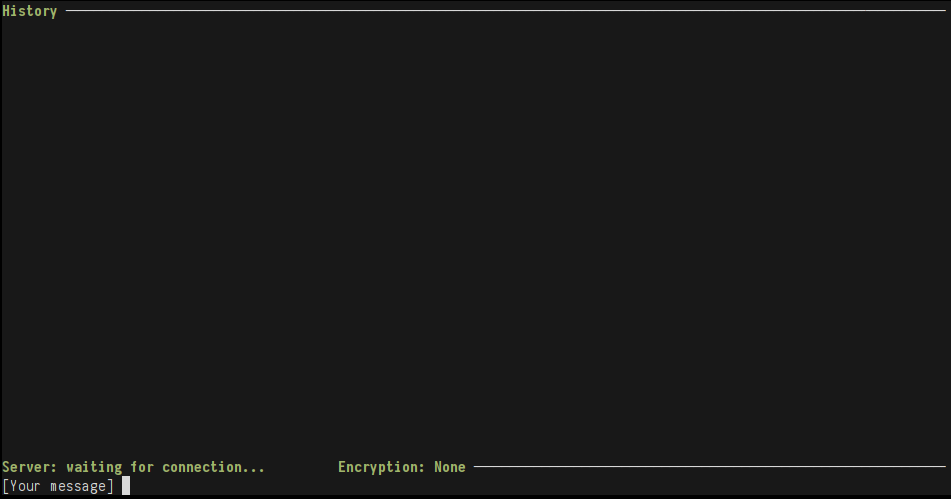
\includegraphics[scale=0.4]{podstawowy_interfejs_po_uruchomieniu_serwer}
        \caption{Interfejs aplikacji ,,Bob'' uruchomionej jako serwer}
        \label{SERVER_INTERFACE}
    \end{figure}
    \begin{figure}[tp]
        \centering
        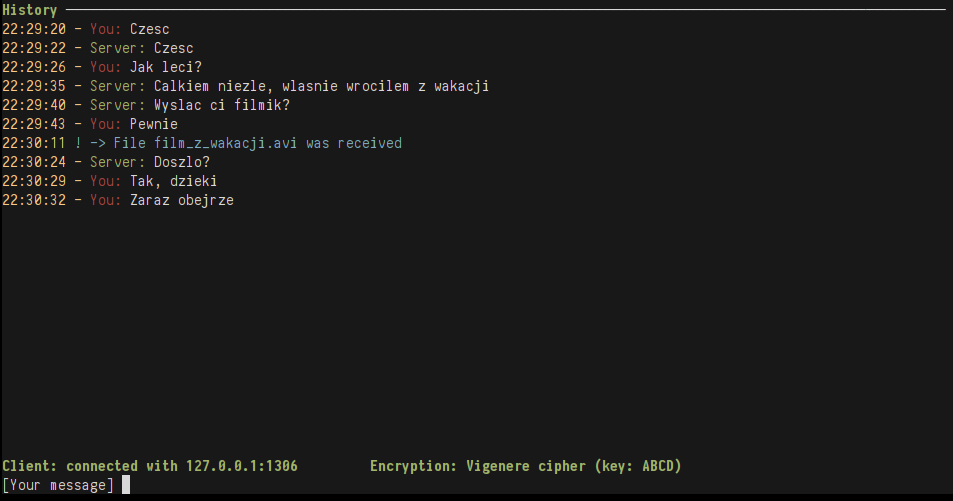
\includegraphics[scale=0.4]{interfejs_podczas_dzialania_klient}
        \caption{Interfejs aplikacji ,,Bob'' w trakcie działania jako klient}
        \label{CLIENT_INTERFACE}
    \end{figure}
    \subsubsection{Pasek stanu}
      Pasek stanu zawiera informacje na temat aktualnego statusu aplikacji. Znajdują się tutaj informacje na temat
      połączenia oraz aktualnie wykorzystywanego szyfrowania
    \subsubsection{Okienko do wpisywania wiadomości}
      Domyślnie aktywne po uruchomieniu aplikacji. Możliwe jest tutaj wpisanie treści wiadomości do przekazania
      rozmówcy. Po wpisaniu wiadomości jej wysłanie odbywa się po wciśnięciu klawisza \emph{Enter}
    \subsubsection{Historia rozmowy}
      W oknie tym wyświetlone są wszystkie wiadomości odebrane oraz wysłane. Każda wiadomość opisana jest godziną
      wysłania (odebrania) oraz nadawcą. Możliwe jest aktywowanie okna historii poprzez naciśnięcie klawisza
      \emph{Tab}. Po aktywowaniu, możliwe jest wybieranie wiadomości. Po naciśnięciu klawisza \emph{Enter} na
      wybranej wiadomości wyświetlone zostanie okienko ze szczegółami wiadomości. Możliwe jest tutaj sprawdzenie
      szyfrowania, które zostało użyte do wysłania wiadomości oraz podejrzenie powstałego szyfrogramu oraz tekstu
      jawnego.

      Oprócz wysłanych oraz odebranych wiadomości w oknie historii rozmowy wyświetlane są również informacje na
      temat odebranych oraz wysłanych plików. Podobnie jak w przypadku wiadomości możliwe jest wybranie dowolnego
      z tych wpisów oraz po naciśnięciu klawisza \emph{Enter} podejrzenie szczegółów transmisji plików.

    \begin{figure}[H]
        \centering
        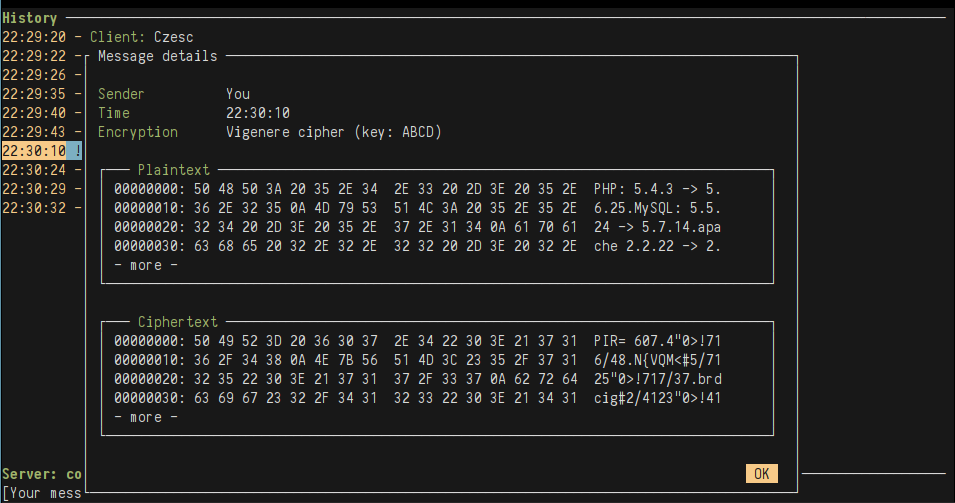
\includegraphics[scale=0.4]{szczegoly_transferu_pliku}
        \caption{Okienko przedstawiające szczegóły transferu pliku}
        \label{FILE_TRANSFER_DETAILS}
    \end{figure}

      W zależności od wykorzystywanego szyfrowania oraz od tego czy wybrana została wiadomość czy transfer pliku,
      szyfrogram oraz tekst jawny mogą zostać przedstawione w postaci zwykłego tekstu lub w postaci szesnastkowej.

    \subsubsection{Menu aplikacji}
      Menu aplikacji otwierane jest po naciśnięciu klawiszy \emph{CTRL + X}

    \begin{figure}[H]
        \centering
        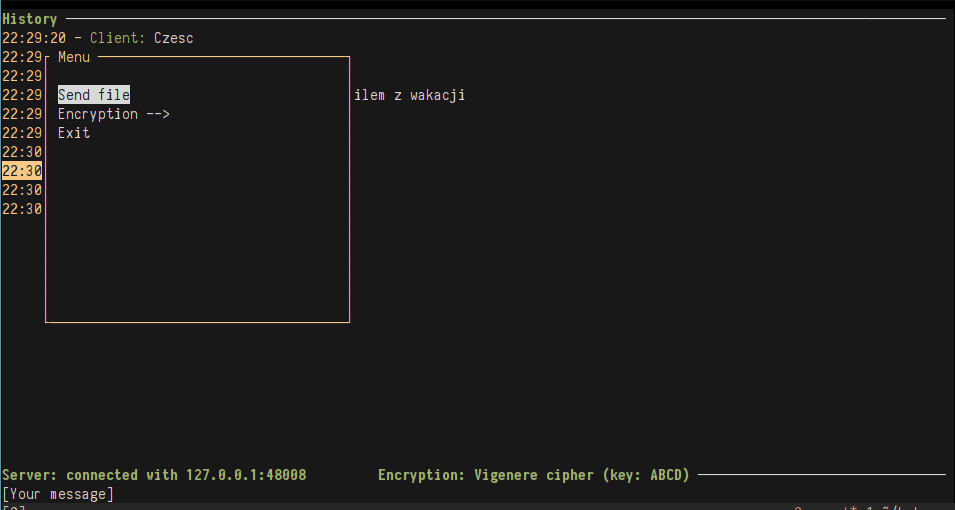
\includegraphics[scale=0.4]{menu_aplikacji}
        \caption{Menu aplikacji}
        \label{APPLICATION_MENU}
    \end{figure}

    \paragraph{Wysyłanie pliku}
      Po wybraniu opcji \emph{Send file} możliwe jest wysłanie pliku do rozmówcy. W wyświetlonym oknie należy za
      pomocą strzałek wybrać odpowiedni plik, po czym zatwierdzić wybór klawiszem \emph{Enter}. W tym momencie
      rozmówca zostaje poproszony o akceptację transferu pliku, oraz wskazanie lokalizacji zapisu pliku, przy
      pomocy analogicznego okna dialogowego. Po akceptacji rozpoczna się transmisja pliku, której postęp
      przedstawiony jest w~wyświetlonym okienku.

    \begin{figure}[h]
        \centering
        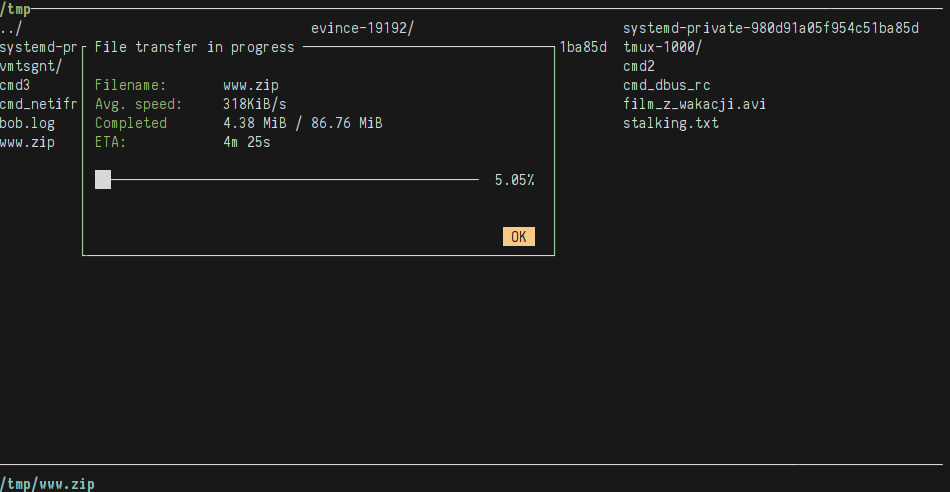
\includegraphics[scale=0.4]{transfer_pliku}
        \caption{Okieno pokazujące postęp transmisji pliku}
        \label{FILE_TRANSFER_PROGRESS}
    \end{figure}

    \paragraph{Zmiana sposobu szyfrowania}
      Przy pomocy opcji \emph{Encryption} możemy wybrać sposób szyfrowania przesyłanych wiadomości oraz plików.
      Po wybraniu tej opcji w kolejnym menu zaprezentowane są dostępne sposoby szyfrowania. Po wybraniu dowolnego z
      nich wyświetlone zostaje okienko konfiguracji szyfrowania. W zależności od wybranego algorytmu należy podać
      odpowiedni klucz. Po zatwierdzeniu przyciskiem \emph{OK} szyfrowanie będzie aplikowane do wysłanych oraz
      odebranych wiadmości. Informacja o wykorzystywaniu szyfrowania zostaje wysłana do rozmówcy, dzięki czemu nie
      jest konieczne ponowne konfigurowanie algorytmu, zostaje on ustawiony automatycznie

    \begin{figure}[H]
        \centering
        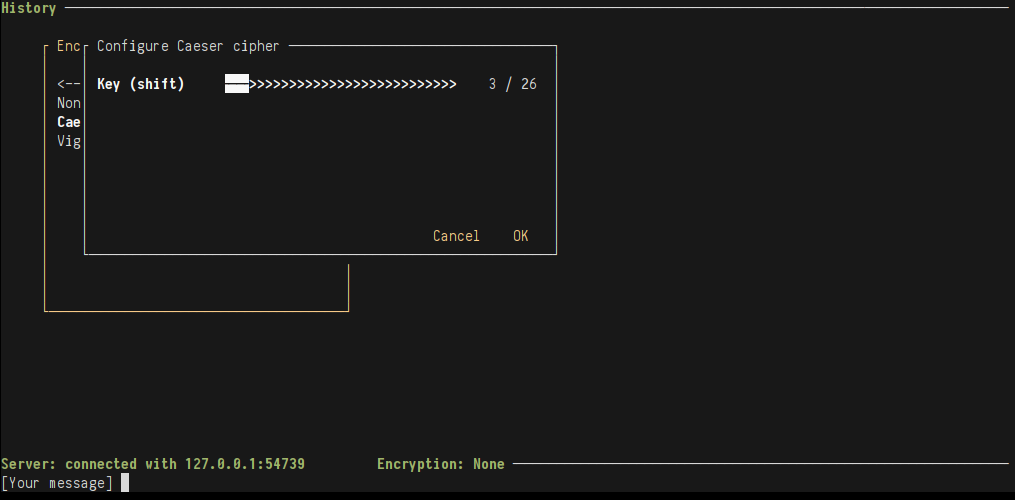
\includegraphics[scale=0.4]{caesar_cipher_configuration}
        \caption{Okienko konfiguracji szyfru Cezara}
        \label{CIPHER_CONFIGURATION}
    \end{figure}

    \paragraph{Wyjście z aplikacji}
      Po wybraniu opcji \emph{Exit} aplikacja zostaje zamknięta. Do rozmówcy zostaje wysłana informacja o
      zerwaniu połączenia, w~związku z czym jego aplikacja również zostaje zamknięta

  \section{Szczegóły implementacji}
    \subsection{Algorytmy szyfrowania}
    Klasy w których zaimplementowana została logika związana z szyfrowaniem znajdują się w folderze \emph{encryption}.
    \begin{itemize}
            \item \emph{base.py} - znajdują się tutaj klasy bazowe, które dostarczają implementację metod pomocniczych
            \item \emph{ciphers.py} - zaimplementowane są tutaj konkretne szyfry, które mogą być wykorzystywane podczas
                transmisji plików oraz wiadomości
    \end{itemize}

    \begin{figure}[H]
        \centering
        \includegraphics[scale=0.6]{cryptography_uml}
        \caption{Diagram klas związanych z szyfrowaniem}
        \label{CRYPTOGRAPHY_UML}
    \end{figure}

    \subsubsection{Klasy bazowe}

      \begin{itemize}
          \item {\bfseries CipherWithoutKey} - Klasa bazowa dla szyfrów, które nie posiadają klucza, bądź klucz jest
              z góry ustawiony zaimplementowana jest tutaj serializacja oraz deserializacja parametrów tych szyfrów do
              celów ustalenia sposobu szyfrowania pomiędzy serwerem a klientem, jedynym przesyłanym parametrem jest
              nazwa algorytmu szyfrowania.
          \item {\bfseries SingleKeyCipher} - Klasa bazowa dla szyfrów posiadających jeden klucz, serializacja i
              deserializacja takich szyfrów obejmuje zarówno nazwę algorytmu jak i używany klucz.
          \item {\bfseries ShiftBasedCipher} - Klasa bazowa dla szyfrów opartych o zastępowanie poszczególnych liter
              tekstu jawnego inną literą oddaloną o określoną liczbę pozycji w alfabecie. Zaimplementowane są dwie
              metody pomocnicze:
              \begin{itemize}
                  \item \emph{\_shift\_character} - przesuwa znak o określoną liczbę pozycji uwzględniając z jakiego
                      zbioru on pochodzi tzn. małe litery przesuwane są jedynie wśród małych liter, wielkie litery wśród
                      wielkich liter, natomiast cyfry wśród cyfr. Oznacza to, że litera 'z' przesunięta o jedną pozycję
                      staje się literą 'a', a litera 'Z' staje się literą 'A'. Znaki, które nie są literą ani cyfrą nie
                      są szyfrowane.
                   \item \emph{\_shift\_binary\_charater} - przesuwając każdy znak traktuje go jako znak binarny
                       pochodzący z 256-znakowego alfabetu.
              \end{itemize}
      \end{itemize}

    \subsubsection{Zaimplementowane szyfry}
      Każda klasa implementująca szyfr posiada odpowiednie metody
      \begin{itemize}
          \item \emph{encrypt} - metoda szyfrująca tekst jawny składający się ze znaków alfanumeryczych
          \item \emph{decrypt} - metoda deszyfrująca szyfrogram zaszyfrowany wcześniej metodą \emph{encypt}
          \item \emph{encrypt\_binary} - metoda szyfrująca tekst jawny składający się z bajtów
          \item \emph{decrypt\_binary} - metoda deszyfrująca szyfrogram zaszyfrowany wcześniej metodą \emph{encypt\_binary}
      \end{itemize}

      Zaimplementowane algorytmy szyfrowania to:
      \begin{itemize}
          \item {\bfseries NoneEncryption} - Klasa implementująca wzorzec projektowy \emph{Null Object Patern}, używana
              gdy szyfrowanie nie jest aktywne, wszystkie jej opisane powyżej metody zwracają tekst jawny oraz szyfrogram
              w dokładnie takiej samej formie jak podana na wejściu.
          \item {\bfseries CaesarCipher} - Klasa implementująca szyfr Cezara, parametryzowana kluczem.
          \item {\bfseries Rot13Cipher} - Klasa implementująca szyfr Rot13, dziedziczy z klasy CaesarCipher, wprowadza
              na stałe ustalony klucz.
          \item {\bfseries ViegenreCipher} - Klasa implementująca szyfr Viegenere, dostarczony klucz musi składać się
              wyłącznie z wielkich liter. Przesunięcie kolejnego znaku tekstu jawnego odpowiada pozycji w alfabecie kolejnego
              znaku klucza, w razie potrzeby klucz jest zapętlany.
          \item {\bfseries AESCipher} - Klasa implementujące algorytm szyfrowania AES, wykorzystana została implementacja
              dostarczana przez bibliotekę \emph{cryptography} napisaną w języku Python.
      \end{itemize}

    \subsubsection{Implementacja szyfru AES}
      Do implementacji szyfru AES została wykorzystana biblioteka \emph{cryptography} napisana w języku Python. Biblioteka
      ta dostarcza zarówno klasę implementującą szyfr AES, klasy implementujące różnego rodzaju tryby wiązania oraz
      klasy implementujące różne strategie dopełnianie niepełnych bloków, które mają być zaszyfrowane (padding).

      Klasa \emph{Cipher} pozwala połączyć szyfr blokowy z wybranym trybem wiązania. Udostępnia ona dwie metody
      \emph{encryptor} oraz \emph{decryptor}. Zwracają one obiekt kontekstu szyfrowania, który posiada metodę \emph{update}
      pozwalającą na podawanie kolejnych porcji danych do zaszyfrowania/odszyfrowania oraz zwracającą pełne bloki
      szyfrogramu/tekstu jawnego. Dane, które nie tworzą pełnego bloku są buforowane wewnątrz kontekstu szyfrowania.
      Aby uzyskać końcówkę zaszyfrowanych danych należy wywołać metodę \emph{finalize}

      Szyfry blokowe wymagają aby długość tekstu jawnego oraz szyfrogramu zawsze była wielokrotnością długości bloku
      danego szyfru blokowego. Z tego powodu, niekiedy potrzebne jest dopełnienie wiadomości do rozmiaru bloku (padding).
      Kontekst szyfrowania domyślnie nie aplikuje żadnego dopełnia do przekazywanych do niego bloków. Z tego powodu
      w klasie AESCipher zostało zaimplementowane dopełnianie niezależne od kontekstu szyfrowania. Dopełniana jest
      każda wiadomość tekstowa oraz plik przesyłany pomiędzy klientem a serwerem. Do dopełniania bloków wykorzystany został
      algorytm PKCS7.

      Interfejs konfiguracji algorytmu AES pozwala na podanie przez użytkownika zarówno klucza jak i wektora incjującego
      dla trybu wiązania CBC. Akceptowane są wszystkie dozwolone dla algorytmu AES długości klucza (16, 24, 32 bajty).
      Okienko konfiguracyjne pozwala zarówno na ręczne wprowadzenie wymaganych wartości przez użytkownika jak i na ich
      losowe wygenerowanie. Wektor inicjujący jest przesyłany do rozmówcy w wiadomości mówiącej o zmianie wykorzystywanego
      sposobu szyfrowania. Ten sam wektor inicjujący jest wykorzystywany do czasu zmiany go przez użytkownika bądź zmiany
      wykorzystywanego szyfrowania.

    \subsubsection{Implementacja szyfru RSA}
      \paragraph{Opis algorytmu RSA}
        Algorytm RSA jest asymetrycznym algorytmem szyfrowania, co oznacza, że wykorzystuje on dwa powiązane ze sobą
        klucze umożliwiające przeprowadzanie operacji szyfrowania i deszyfrowania. Wśród tych kluczy wyróżniony jest
        klucz prywatny, który jak sama nazwa mowi powinien być utrzymany w tajemnicy, oraz klucz publiczny, który
        udostępniany jest każdemu zainteresowanemu. Klucza prywatnego nie można w łatwy sposób odtworzyć z klucza
        publicznego. Klucz publiczny jest używany do zaszyfrowania informacji, natomiast klucz prywatny do jej odszyfrowania.
        Jedynie adresat może odczytać wiadomość, ponieważ jedynie on ma dostęp do klucza prywatnego. W algorytmie RSA
        bezpieczeństwo szyfrowania opiera się na trudności faktoryzacji dużych liczb złożonych.  W celu wygenerowania
        pary kluczy należy:
        \begin{itemize}
          \item Wybrać losowo dwie duże liczby pierwsze \emph{p} i \emph{q}
          \item Obliczyć wartość \( n = p * q \)
          \item Obliczyć wartość \( \phi = (p - 1) * (q - 1) \)
          \item Wybrać liczbę \emph{e} względnie pierwszą z \( \phi \)
          \item Znaleźć liczbę \emph{d}, gdzie jej różnica z odwrotnością liczby \emph{e} jest podzielna przez \( \phi \)
      \end{itemize}
      Po wykonaniu powyższych kroków liczby \( (n,e) \) stanowią klucz publiczny, a liczby \( (n,d) \) klucz prywatny. \\
      Szyfrowanie polega na obliczeniu liczby \( c = t^e\mod n \) \\
      Deszyfrowanie polega na obliczeniu liczby \( t = c^d\mod n \)

      \paragraph{Własna implementacja szyfru RSA}
        Własna implementacja szyfru RSA została umieszczona w klasie \emph{SzacunProductionRSACipher} w pliku
        \emph{encryption/ciphers.py}.
        Może zostać ona uaktywniona poprzez jej wybranie w~menu aplikacji, jak opisano powyżej. Wielkość bloku szyfrowania
        ustalana jest na podstawie długości używanego klucza, jeśli długość klucza w bajtach wynosi \emph{n}, to długość
        bloku tekstu jawnego wynosi \( n - 1 \). Ostatni blok wiadomości jest dopełniany w razie potrzeby, zgodnie z
        algorytmem PKCS7. Każdy blok składający się z bajtów zamieniany jest na liczbę całkowitą,
        która szyfrowana jest zgodnie z opisaną powyżej procedurą szyfrowania algorytmu RSA. Wynikiem szyfrowania jest
        liczba, która zostaje z powrotem zamieniona na ciąg bajtów, o~długości odpowiadającej długości bloku szyfrogramu,
        czyli \emph{n}. W razie potrzeby liczba dopełniana jest zerami z przodu.

        Zaszyfrowany blok szyfrogramu zostaje przesłany do rozmówcy, tam zostaje on zamieniony na liczbę i poddany
        procedurze odszyfrowania opisanej powyżej, a następnie zamieniany z powrotem na ciąg bajtów. Otrzymany blok tekstu
        jawnego jest w razie potrzeby oczyszczany z dopełnienia.

      \paragraph{Biblioteczna implementacja szyfru RSA}
        Biblioteczna implementacja szyfru RSA znajduje się w klasie \emph{LibraryRSACipher} w pliku \emph{encryption/ciphers.py}.
        Została tutaj wykorzystana wcześniej opisywana bibliotek cryptography napisana w języku Python. Do dopełniania
        bloków został wybrany algorytm OAEP, w którym jako funkcja skrótu wykorzystany został algorytm SHA1. Dopełnienie
        to nakłada ograniczenie na rozmiar bloku tekstu jawnego:
        \begin{equation}
            M_{len} = n - 2 * H_{len} - 2
        \end{equation}
        gdzie \emph{n} to długość używanego klucza, a \( H_{len} \) to długość skrótu, w przypadku SHA1 20 bajtów.
        Biblioteka cryptography nie zapewnia dzielenia wiadomości na bloki, w związku z czym podział na bloki odpowiedniej
        wielkość został zaimplementowany samodzielnie.

        \paragraph{Używanie szyfrowania RSA}
        Szyfrowanie RSA w aplikacji Bob może zostać wykorzystane na dwa sposoby:
        \begin{enumerate}
          \item Do szyfrowania wszystkich przesyłanych wiadomości oraz plików - w tym celu należy z menu Encrpytion
            wybrać odpowiednią opcję: SzacunProductionRSACipher aby uaktywnić własną implementację szyfru RSA,
            bądź LibraryRSACipher, aby wykorzystać implementację biblioteczną.
          \item Do zaszyfrowania klucza algorytmu AES - w tym celu z menu Encryption należ wybrać opcję AESCipher,
            a następnie w okienku konfiguracyjnym po wpisaniu, bądź wygenerowaniu klucza zaznaczyć opcję
            ,,Send key using RSA''. Do zaszyfrowania klucza algorytmu AES zawsze wykorzystywana jest własna
            implementacja algorytmu RSA. Po wybraniu tej opcji, klucz sesyjny zostaje w postaci zaszyfrowanej
            wysłany do rozmówcy, gdzie następuje jego odszyfrowanie i automatyczne uaktywnienie odpowiedniego szyfrowania.
        \end{enumerate}
        Wymiana kluczy publicznych między klientem a serwerem następuje zaraz po uzyskaniu połączenia. Najpierw swój
        klucz do klienta wysyła serwer, a następnie klient jako odpowiedź wysyła swój klucz publiczny. Dzięki tej
        procedurze odpowiednie klucze publiczne dostępne są w każdej chwili i mogą zostać wykorzystane zarówno
        do szyfrowania wszystkich wiadomości i plików jak i do szyfrowania kluczy sesyjnych

  \subsection{Porównanie wydajności algorytmów szyfrowania}
    Badania zostały przeprowadzone przy wykorzystaniu następujących parametrów:
    \begin{itemize}
      \item Długość klucza RSA: \( 2048 \) bitów
      \item Długość klucza AES: \( 256 \) bitów
      \item Rozmiar przesyłanego pliku: \( 15000000 \) bajtów \( = 14,36 \) megabajtów
    \end{itemize}

    \begin{center}
      \begin{tabular}{ | l | l |}
      \hline
      Nazwa algorytmu & Czas transferu pliku \\ \hline
      AESCipher & 1 sekunda \\ \hline
      LibraryRSACipher & 2 minuty 34 sekundy \\ \hline
      SzacunProductionRSACipher & 12 minut 3 sekundy  \\ \hline
      \end{tabular}
    \end{center}

    \begin{figure}[H]
        \centering
        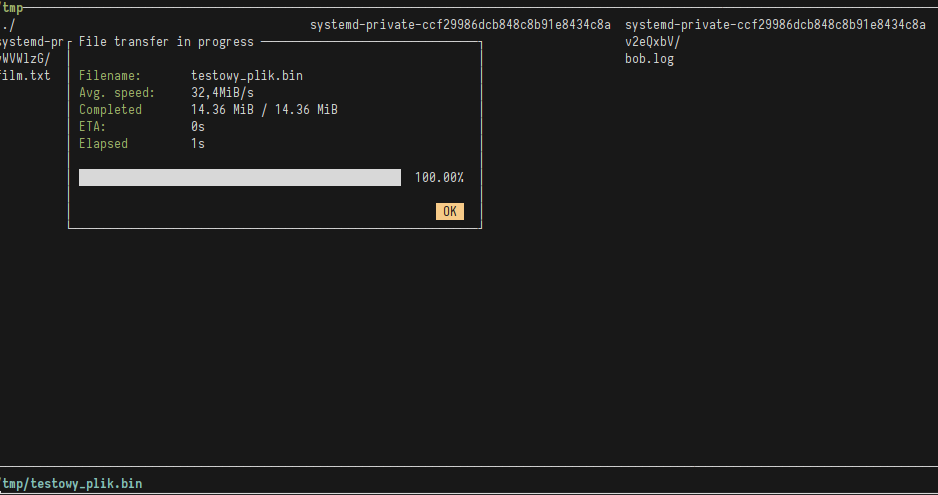
\includegraphics[scale=0.4]{aes_cipher}
        \caption{Transfer pliku z wykorzystaniem algorytmu AES}
        \label{AES_FILE_TRANSFER}
    \end{figure}
    \begin{figure}[H]
        \centering
        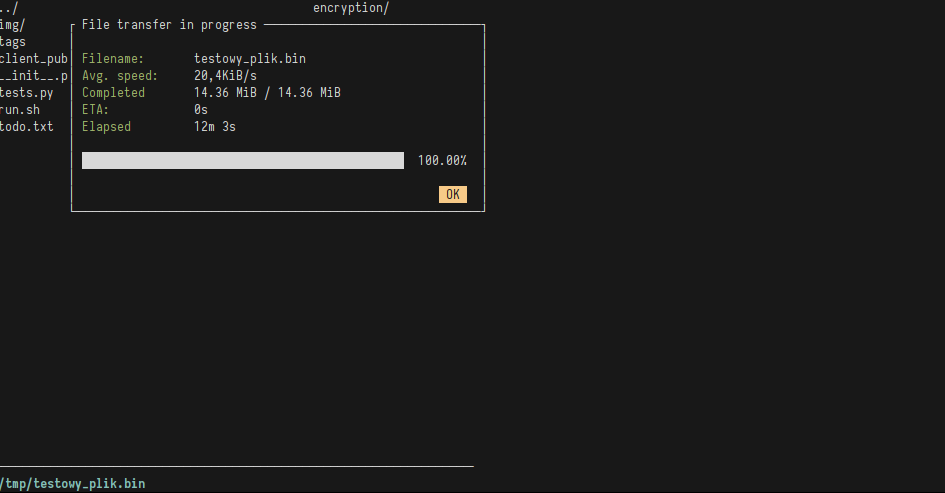
\includegraphics[scale=0.4]{szacun_production_rsa}
        \caption{Transfer pliku z wykorzystaniem własnej implementacji algorytmu RSA}
        \label{SZACUN_RSA_FILE_TRANSFER}
    \end{figure}
    \begin{figure}[H]
        \centering
        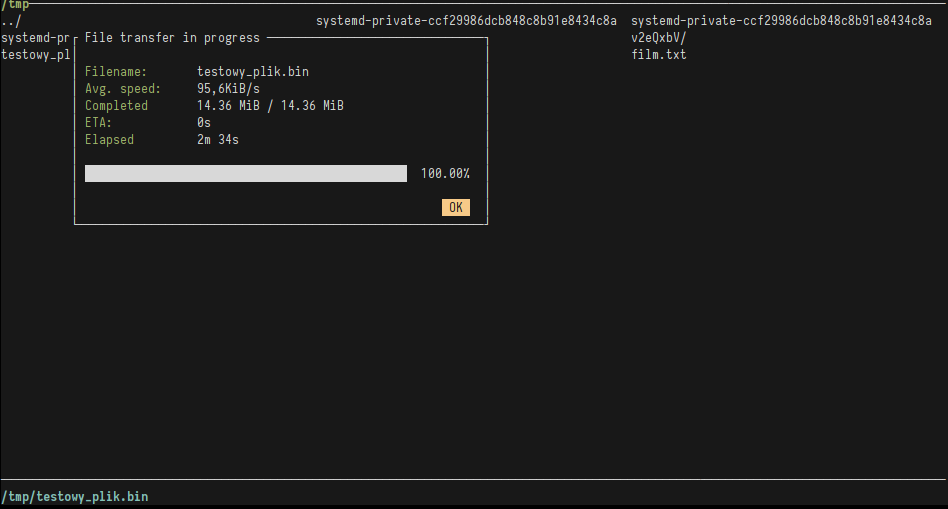
\includegraphics[scale=0.4]{library_rsa_cipher}
        \caption{Transfer pliku z wykorzystaniem bibliotecznej implementacji algorytmu RSA}
        \label{LIBRARY_RSA_FILE_TRANSFER}
    \end{figure}


  \subsection{Interfejs użytkownika}
  Klasy związane z interfejsem użytkownika znajdują się w folderze \emph{gui}. Wśród ważniejszych klas można wyróżnić:
  \begin{itemize}
      \item {\bfseries MainWindow} (main\_window.py) - Klasa implementująca główne okno aplikacji, zawarte są w niej
          wszystkie widgety widoczne w głównym oknie, zajmuje się ona tworzeniem oraz obsługą menu programu. Klasa ta
          otrzymuje od protokołu sieciowego informacje o wszelkich zdarzeniach i odpowiednio je obsługuje, na przykład
          wyświetla wiadomości w oknie z historią, pyta użytkownika o zgodę na odebranie pliku oraz wyświetla informacje
          o~zmianie sposobu szyfrowania zaproponowanej przez rozmówcę.
      \item {\bfseries HistoryRemeberingTextCommandBox} (command\_box.py) - Klasa implementująca okienko do wpisywania
          wiadomości przeznaczonej do wysłania. Zawiera logikę wyświetlającą tekst zachęty (,,[Your message]'') oraz
          pozwala na używanie strzałek góra/dół do ponownego wysłania tej samej wiadmości.
      \item {\bfseries MessageHighlightMultiLine} (highlighting.py) - Klasa implementująca historię rozmowy,
          zaimplementowane zostało tutaj odpowiednie formatowanie wiadomości oraz kolorowanie poszczególnych jej części
          na przykład czasu otrzymania oraz autora. Ponadto obsługiwany jest klawisz \emph{Enter} pozwalający wyświetlić
          szczegóły wybranej wiadomości.
      \item Okienka dialogowe znajdujące się w katologu \emph{gui/popups}:
      \begin{itemize}
          \item {\bfseries CaesarEncryptionConfigurationPopup} (caesar\_encryption\_configuration.py) - Okienko służące
              do konfiguracji szyfru Cezara. Wykorzystuje klasę \emph{IntegerSlider}, która jest kontrolką typu slider,
              zwracającą wartości całkowite.
          \item {\bfseries NotHiddenFileSelector} (file\_select.py) - Okienko służące do wyboru pliku do wysłania, bądź
              lokalizacji zapisu pliku odbieranego. Zaimplementowano ukrywanie plików uznawanych za ukryte w systemach
              UNIX (zaczynających się od kropki).
          \item {\bfseries FileTransferProgressPopup} (file\_transfer\_progress.py) - Okienko służące do wyświetlania postępu
              transferu pliku. Wykorzystana klasa \emph{ProcessBarBox} to nieedytowalny slider, wykorzystany w
              charakterze paska postępu.
          \item {\bfseries MessageDetailsPopup} (message\_details.py) - Okienka wyświetlające szczegóły wybranej przez
              użytkownika wiadomości, korzysta z~klasy \emph{SynchronizedPager} która pozwala użytkownikowi jednocześnie
              przewijać okienko z tekstem jawnym i szyfrogramem, dzięki czemu okienka te pozostają zsynchronizowane i
              zawsze pokazują odpowiadające sobie fragmenty.
      \end{itemize}
  \end{itemize}


\end{document}
